\documentclass[]{article}
\usepackage[utf8x]{inputenc}
\usepackage[russian]{babel}
\usepackage{hyperref}
\usepackage{amsmath}
\usepackage{amssymb}
\usepackage{cancel}
\usepackage{graphicx}
\graphicspath{ {./pictures/} }
\title{Численные методы}
\author{Александр Голованов}

\begin{document}
\maketitle
\newpage
\tableofcontents
\newpage

\section{18 февраля 2025}
\subsection{Графическое решение нелинейных систем}

\subsubsection{Задача 1}

\begin{gather*}
\begin{cases}
3x-y =-10\\
x^2+y=10
\end{cases}
\end{gather*}

\begin{figure}[h]
\caption{Графики задача 1}
\centering
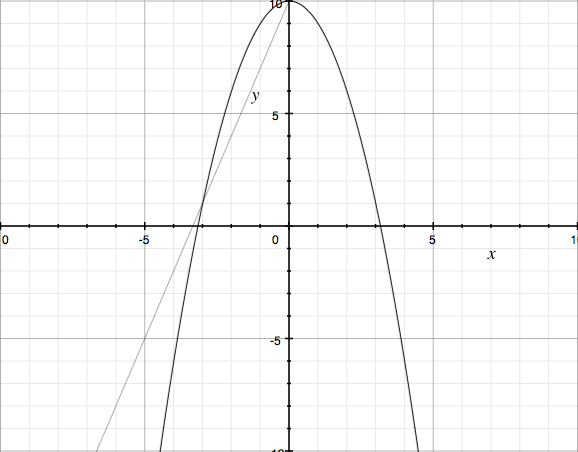
\includegraphics[width=\textwidth]{graph1}
\end{figure}

\subsubsection{Задача 2}

\begin{gather*}
\begin{cases}
x-y =5\\
x*y=6
\end{cases}
\end{gather*}

\begin{figure}[h]
\caption{Графики задача 2}
\centering
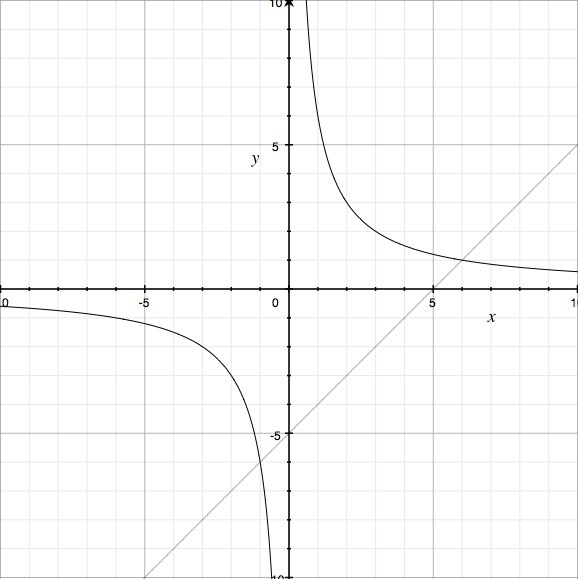
\includegraphics[width=\textwidth]{graph2}
\end{figure}

\subsubsection{Задача 3}

\begin{gather*}
\begin{cases}
x^2+y^2+2xy=9\\
x-y=1
\end{cases}
\end{gather*}

\begin{figure}[h]
\caption{Графики задача 3}
\centering
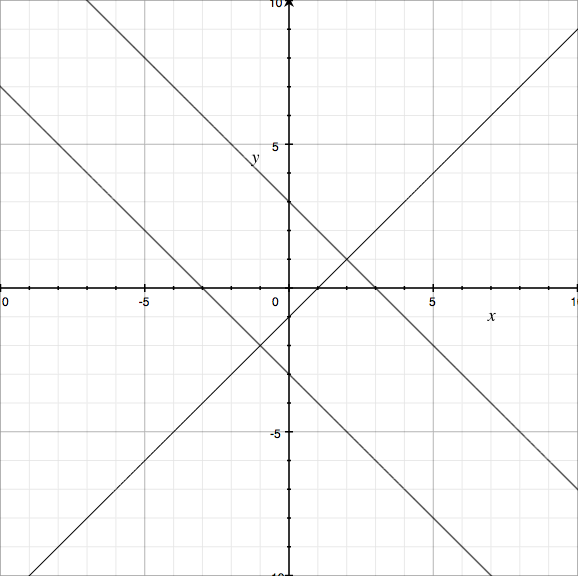
\includegraphics[width=\textwidth]{graph3}
\end{figure}
\end{document}